% !TEX root = ../paper.tex

\section{Evaluation}

This section describes the result of the empiric evaluation of both described algorithms.

\subsection{Single-Writer-Multi-Reader Lock Implementation}

For conducting the expiriments a Sun SPARC T5240 was used, which consists of two UltraSPARC T2 Plus chips with 8 cores each, running at 1.165~GHz. Each core provides 8 hardware threads, for a total of 128 threads (64 per chip). Each run was repeated 5 times. The median was used in the charts. Unfortunately the variance was not quantified in the paper. The throughput was measured in a timespan of 10 seconds. To get stable results the priority queue was seeded with 2000 initial elements. The decision wether to perform an \texttt{add()}-operation or an \texttt{removeMin()}-operation was done randomly with a probability of $p$ resulting in one operation and $1-p$ in the other operation.

The implementation (\textit{pqe}) was compared with 4 other priority queue implementations:
\begin{itemize}
	\item The flat combining skiplist (\textit{fcskiplist}) and the flat combining pairing heap (\textit{fcpairheap}) implementation are both based on the work of \citeauthor{hendler_flat_2010} and use coarse grained locking on a sequential datastructure with flat combining to implement a priority queue algorithm \cite{hendler_flat_2010}.
	\item The lock free skiplist (\textit{lfskiplist}) by \citeauthor{sundell_fast_2003} is based on a parallel skiplist and uses no atomic operations to achieve its lock-freeness. \cite{sundell_fast_2003}.
	\item The Lazy skiplist (\textit{lazyskiplist}) by \citeauthor{lotan_skiplist-based_2000} is based on a parallel skiplist which uses a min-pointer and delete-flags to mark items as taken \cite{lotan_skiplist-based_2000}.
\end{itemize}

The evaluation used different scenarios for evaluating the algorithms by varying the proportion of \texttt{add()} operations and \texttt{removeMin()} operations conversely. In figure~\ref{fig:sparc_50} the results for 50~\% \texttt{add()} and 50~\% \texttt{removeMin()} are shown. The use of elimination suggests a good performance in this scenario. As seen in the diagram, the algorithm \textit{pqe} indeed performs very well. There is a steady increase in throughput up to the maximum thread-count ($60$) tested, but as the throughput seems to level out around 60 threads it can be assumed that the maximum throughput is reached around this number of threads, especially as the machine had to use the second processor for more than 64 threads. The other algorithms reach their peek-throughput between 4 and 8 threads. For low number of threads ($\le 8$) the algorithms is significantly outperformed by \textit{fcpairheap} because of the overhead for elimination and combining in \textit{pqe}.

\begin{figure}[htb]
	\centering
	\begin{minipage}[b]{.495\textwidth}
		\centering
		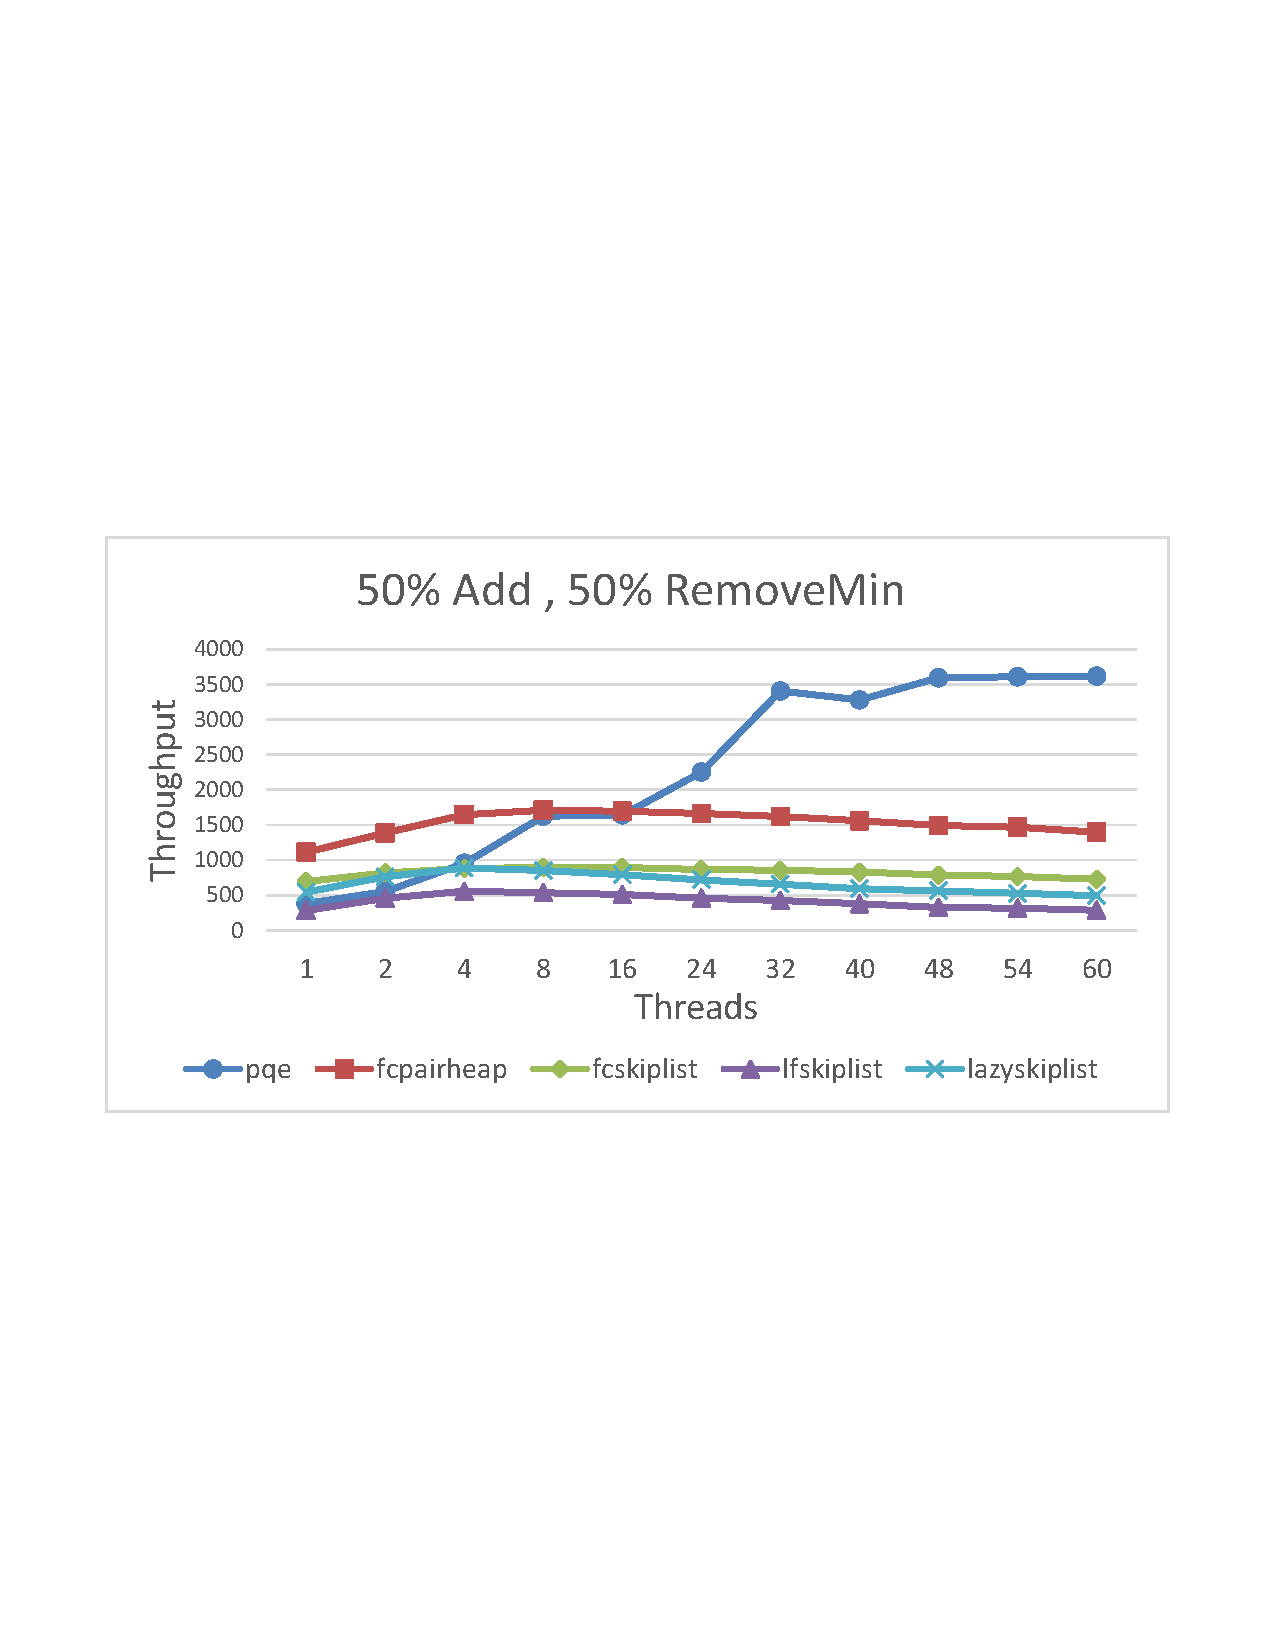
\includegraphics[width=\linewidth]{graphics/sparc-50-50.pdf}
		\caption{Priority queue performance with 50\% \texttt{add()}s, 50\% \texttt{removeMin()}s \cite{calciu_adaptive_2014}.}
		\label{fig:sparc_50}
	\end{minipage}
	\hfill%
	\begin{minipage}[b]{.495\textwidth}
		\centering
		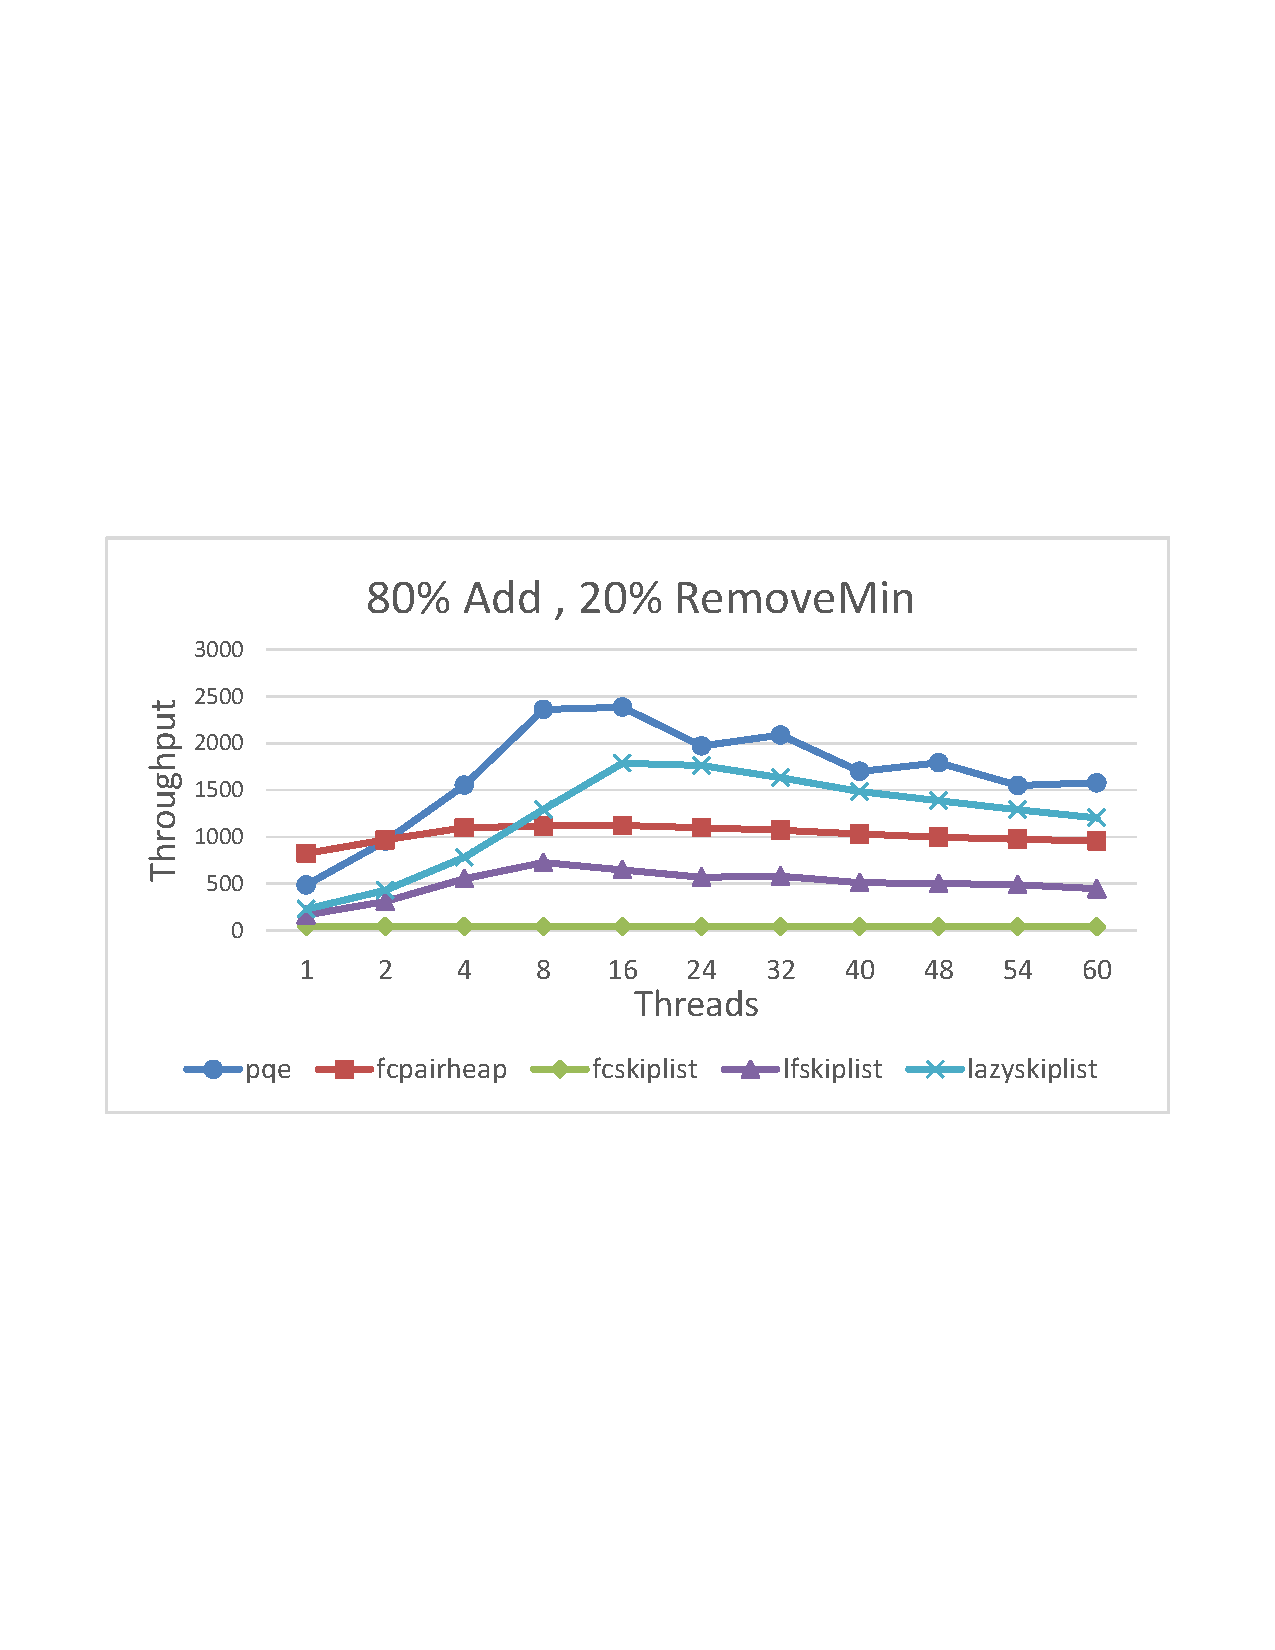
\includegraphics[width=\linewidth]{graphics/sparc-80-20.pdf}
		\caption{Priority queue performance with 80\% \texttt{add()}s, 20\% \texttt{removeMin()}s \cite{calciu_adaptive_2014}.}
		\label{fig:sparc_80}
	\end{minipage}
	\begin{minipage}[b]{.495\textwidth}
		\centering
		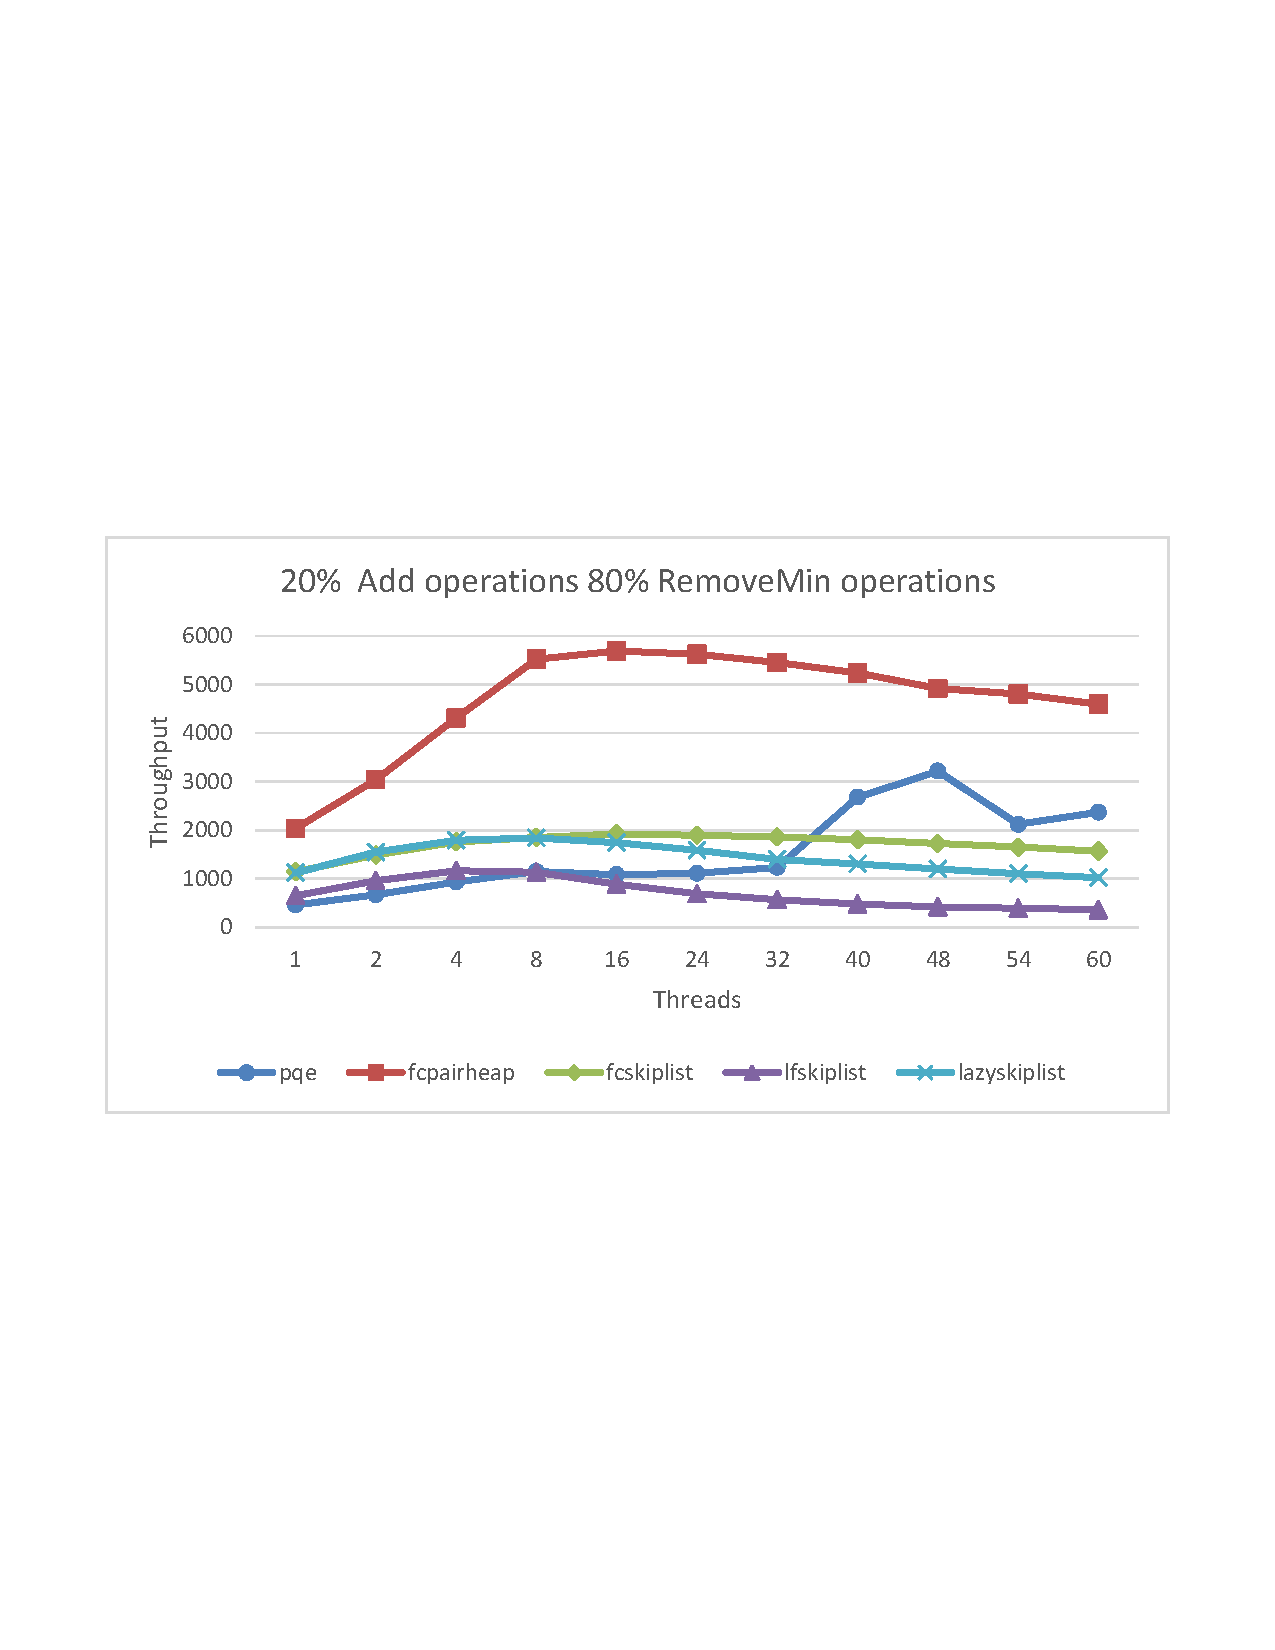
\includegraphics[width=\linewidth]{graphics/sparc-20-80.pdf}
		\caption{Priority queue performance with 20\% \texttt{add()}s, 80\% \texttt{removeMin()}s \cite{calciu_adaptive_2014}.}
		\label{fig:sparc_20}
	\end{minipage}
\end{figure}

Figure~\ref{fig:sparc_80} shows the results for 80~\% \texttt{add()} and 20~\% \texttt{removeMin()}. The use of parallel \texttt{add()} operations still suggests a good performance in this scenario although elimination can't be used that often. Up until 8 threads the \textit{pqe} scales very well with a steady increase in throughput, but from 16 threads on the throughput drops again. The \textit{lazyskiplist} has a similar performance curve, with lower throughput for $\le 16$ threads but a similar decrease from 16 threads on. The curve of \textit{fcpairheap} with a almost static throughput over all tested threadcounts suggests a higher performance than \textit{pqe} and \textit{lazyskiplist} for higher threadcounts than the ones tested. The throughput of about zero for \textit{fcskiplist} seems odd.

The results of the third scenario were not published in the paper by \citeauthor{calciu_adaptive_2014} but the sourcecode located on the \citefield{calciu_adaptive_2014-1}{journaltitle} website contained the results shown in figure~\ref{fig:sparc_20}. The design of the priority queue with sequential \texttt{removeMin()} operations suggests no good performance in this scenario. As seen in the diagram the \textit{pqe} scales quite good with increasing threadcount but has very little throughput in comparison with the other implementations. Other implementations show increasing throughput up to 8 threads, or 16 for \textit{fcpairheap}, but decrease in throughput for higher threadcounts.  Running with $\le 8$ threads \textit{pqe} shows the worst performance of the compared priority queue implementations. \textit{Fcpairheap} outperforms \textit{pqe} by 50~\% to 400~\%. The reason for increasing throughput between 32 and 48 threads is very unexpected and would need further investigation \cite{calciu_adaptive_2014-1}.

In conclusion the \textit{pqe} implementation performs well in scenarios with balanced operation-proportion and in scenarios with more \texttt{add()} operations but has significant performance issues in scenarios with a high \texttt{removeMin()} operation-proportion. This evaluation shows that the implementation by \citeauthor{calciu_adaptive_2014} is no general purpose parallel priority queue and developers still have to evaluate their usecase to find the highest performing priority queue implementation.

\subsubsection{Operation Analysis}

Figure~\ref{fig:sparc_add} shows a diagram breaking down the \texttt{add()} operations optimizations in the different scenarios. While in the first scenario with 80~\% \texttt{add()} operations parallel \texttt{add()} operations account for more than 75~\% of all the \texttt{add()} operations, they only account for about 5~\% in the balanced scenario and none in the third scenario. Operations executed by the server play only a little role as the account for less than 5~\% in the first and second scenario and none in the third. The remaining fraction is executed via elimination.

\begin{figure}[htb]
	\centering
	\begin{minipage}[b]{.495\textwidth}
		\centering
		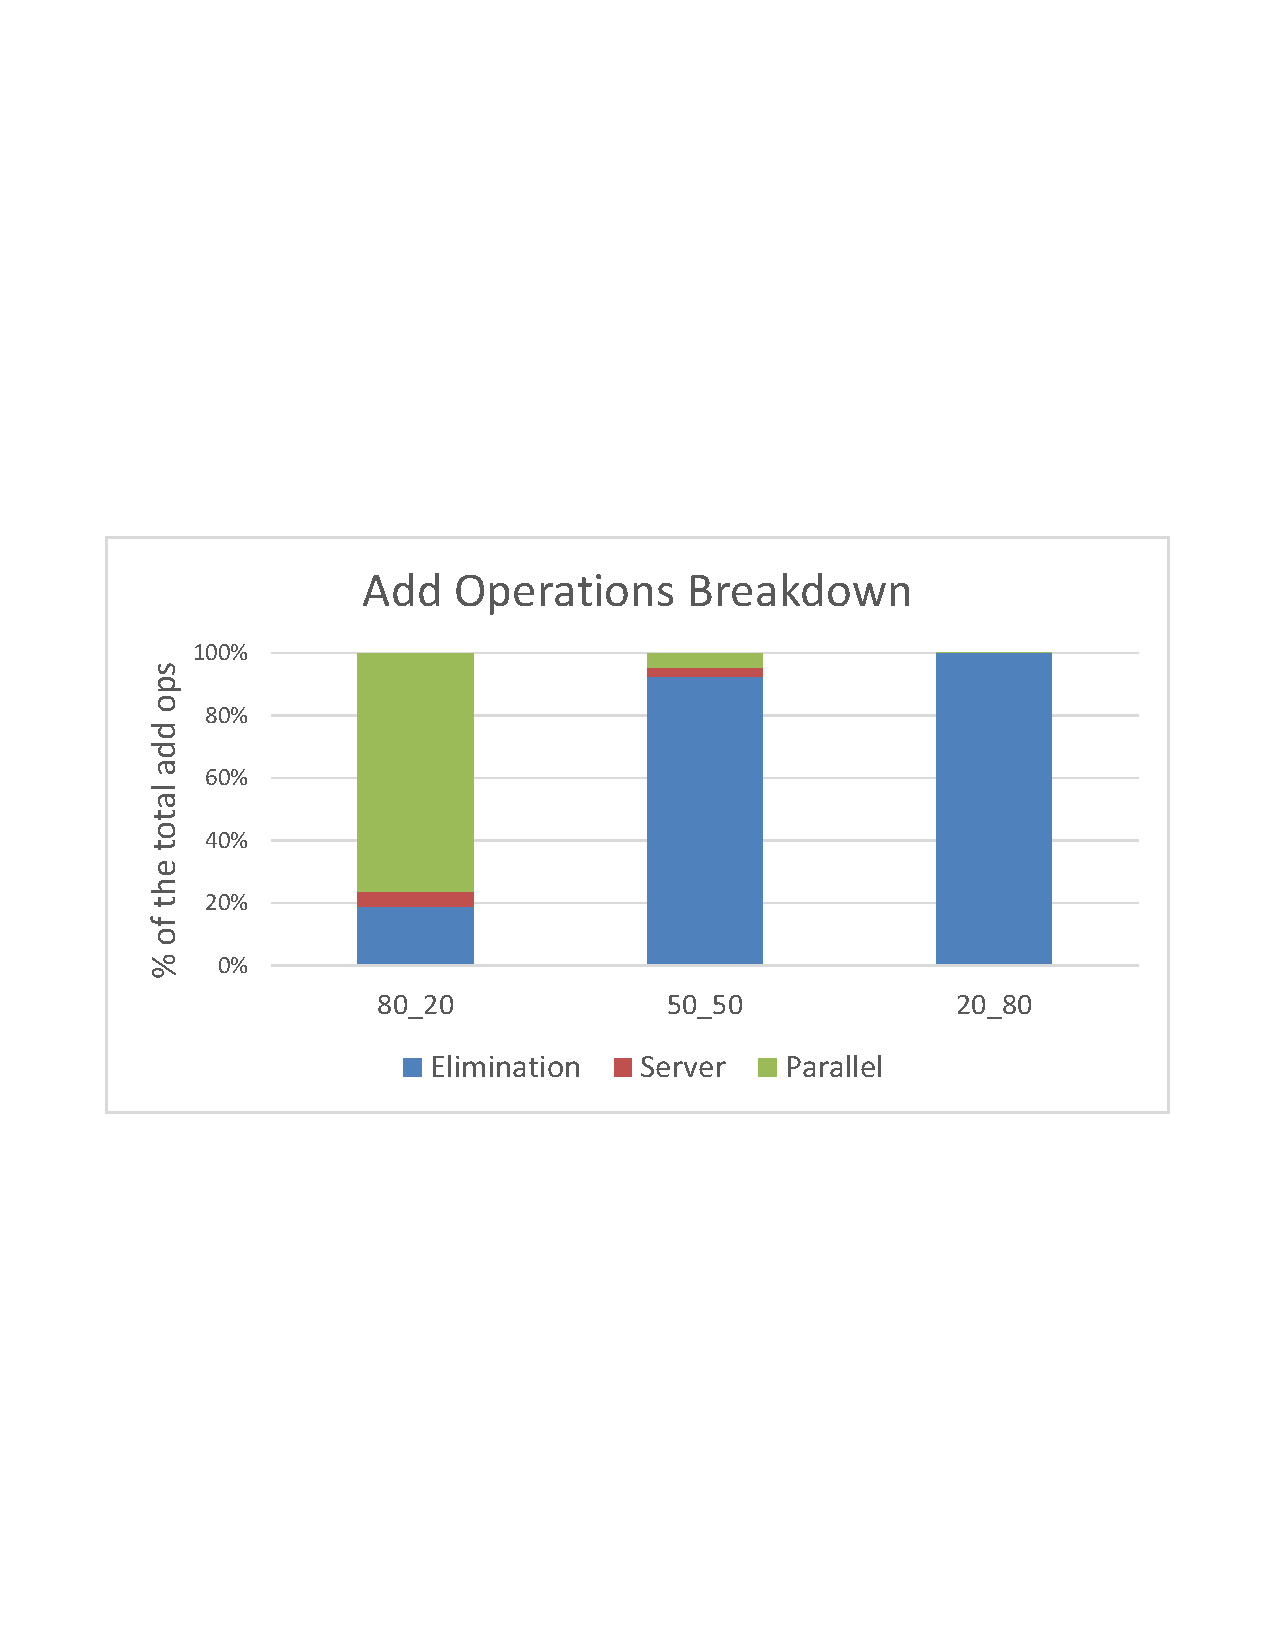
\includegraphics[width=\linewidth]{graphics/sparc-add-brk.pdf}
		\caption{\texttt{add()} work breakdown \cite{calciu_adaptive_2014}.}
		\label{fig:sparc_add}
	\end{minipage}
	\hfill%
	\begin{minipage}[b]{.495\textwidth}
		\centering
		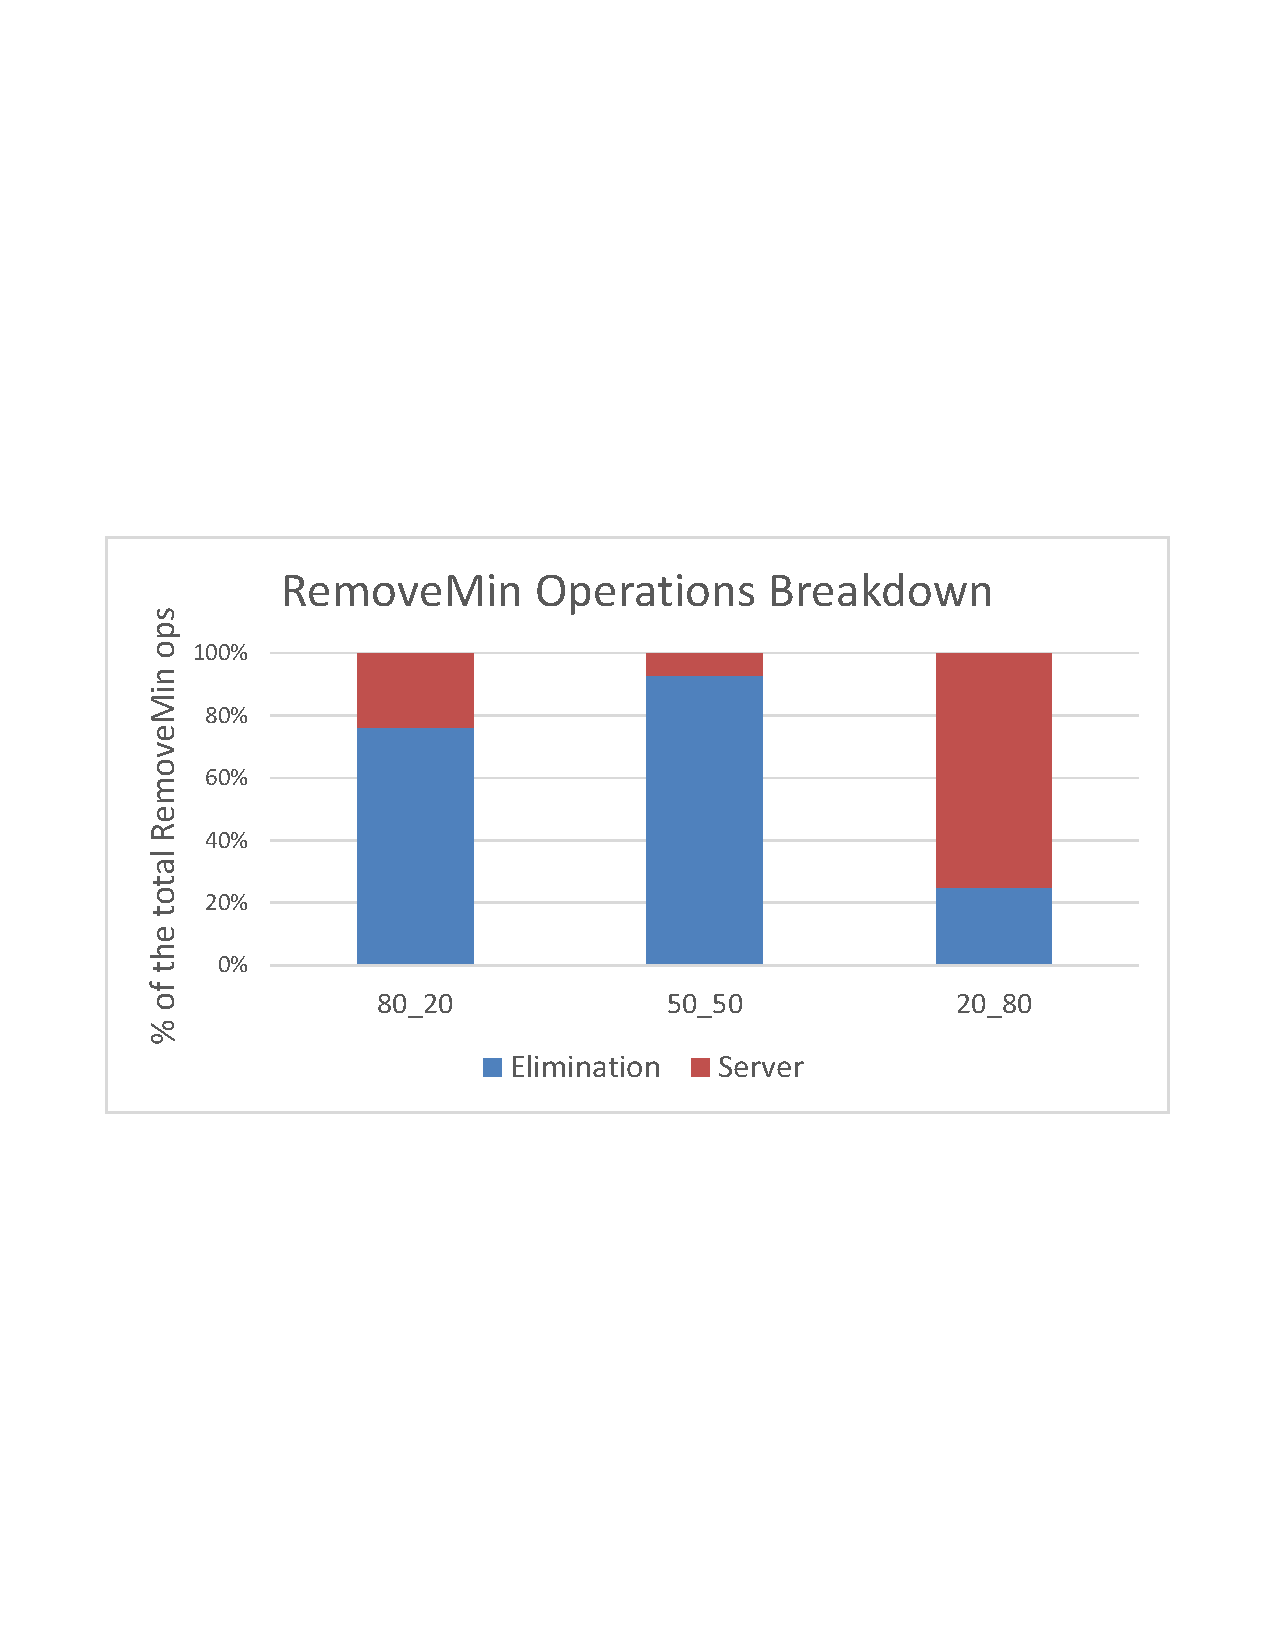
\includegraphics[width=\linewidth]{graphics/sparc-rem-brk.pdf}
		\caption{\texttt{removeMin()} work breakdown \cite{calciu_adaptive_2014}.}
		\label{fig:sparc_rem}
	\end{minipage}
\end{figure}

The \texttt{removeMin()} operations optimizations are shown in figure~\ref{fig:sparc_rem}. In the first scenario with 20~\% \texttt{removeMin()} operations elimination accounts for about 75~\% of all the operations executions. In the balanced scenario elimination accounts for about 90~\% of all the executions while in the last case it's only about 25~\% which explains the low throughput in this scenario as 75~\% of all the \texttt{removeMin()} operations which make up 60~\% of all the operations executed.

\subsection{Hardware Transactional Memory Implementation}

To evaluate the performance of the hardware transactional memory implementation a Intel Core i7-4770 based computer was used. The four cores run at 3.4~GHz and provide two hardware threads each.

, with hardware transactions enabled (restricted transactional memory - RTM),
running at . There are 8GB of RAM shared across the machine and each core has a 32KB L1
cache. Hyperthreading was enabled on our machine so we collected results using all 8 hardware threads.
Hyperthreading causes resource sharing between the hyperthreads, including L1 cache sharing, when running
with more than 4 threads, thus it can negatively impact results, especially for hardware transactions. We
did not notice a hyperthreading effect in our experiments. We used the GCC 4.8 compiler with support for
RTM and optimizations enabled (-O3).

\subsubsection{Aborted Transaction Overhead}

\subsection{Comparison with Algorithm by \citeauthor{braginsky_cbpq:_2016}}

\citeauthor{braginsky_cbpq:_2016} claim in their paper that they implemented a high performing parallel priority queue. They used the original sourcecode by \citeauthor{calciu_adaptive_2014} for conducting their evaluation. The evaluation environment used differs from the one used by \citeauthor{calciu_adaptive_2014}, as they used a machine with 4 16-core AMD Opteron (TM) 6272 processors having a total of 64 threads. The algorithms were all written in C++ and compiled with a -O3 optimization level on Ubuntu~14.04 \cite{braginsky_cbpq:_2016}.

Figures~\ref{fig:cbpq_50}, \ref{fig:cbpq_80} and \ref{fig:cbpq_20} show the results of the conducted experiments to compare the CBPQ algorithm by \citeauthor{braginsky_cbpq:_2016} to other high performing concurrent priority queu implementations at the time. The algorithm by \citeauthor{calciu_adaptive_2014} is abbreviated as APQ in the charts.

\improve{Compare results in detail, focus on low threadcount and scalability especially threadcounts not tested in the original paper}

\begin{figure}[htb]
	\centering
	\begin{minipage}[b]{.7\textwidth}
		\centering
		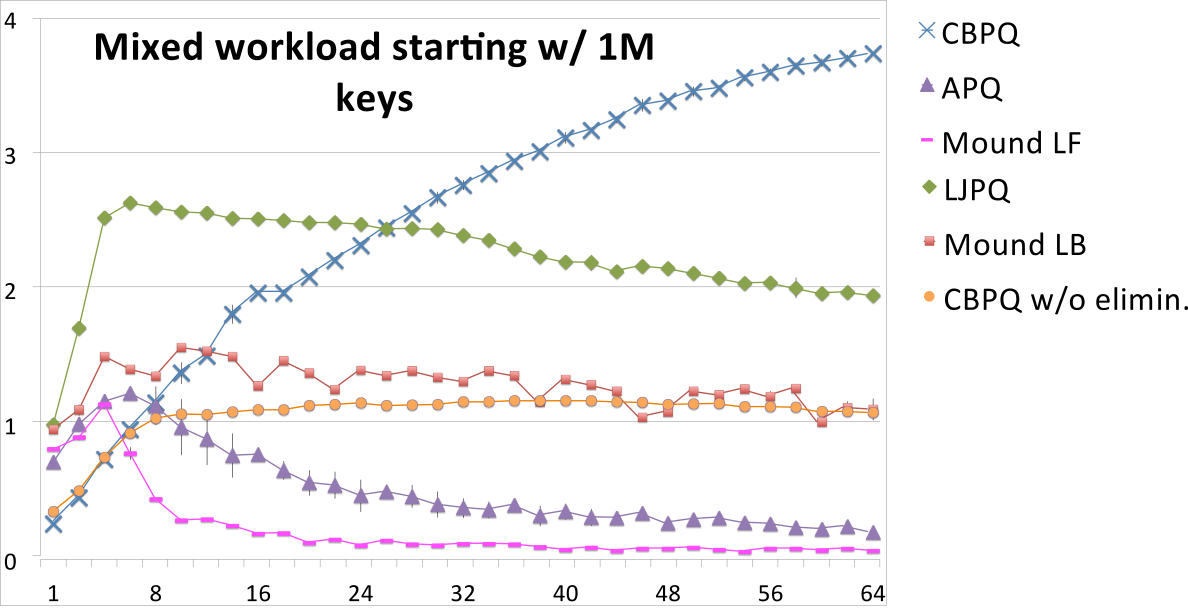
\includegraphics[width=\linewidth]{graphics/cbpq_50add_50.png}
		\caption{Priority queue performance with 50\% \texttt{add()}s, 50\% \texttt{removeMin()}s \cite{braginsky_cbpq:_2016}.}
		\label{fig:cbpq_50}
	\end{minipage}
	\hfill%
	\begin{minipage}[b]{.495\textwidth}
		\centering
		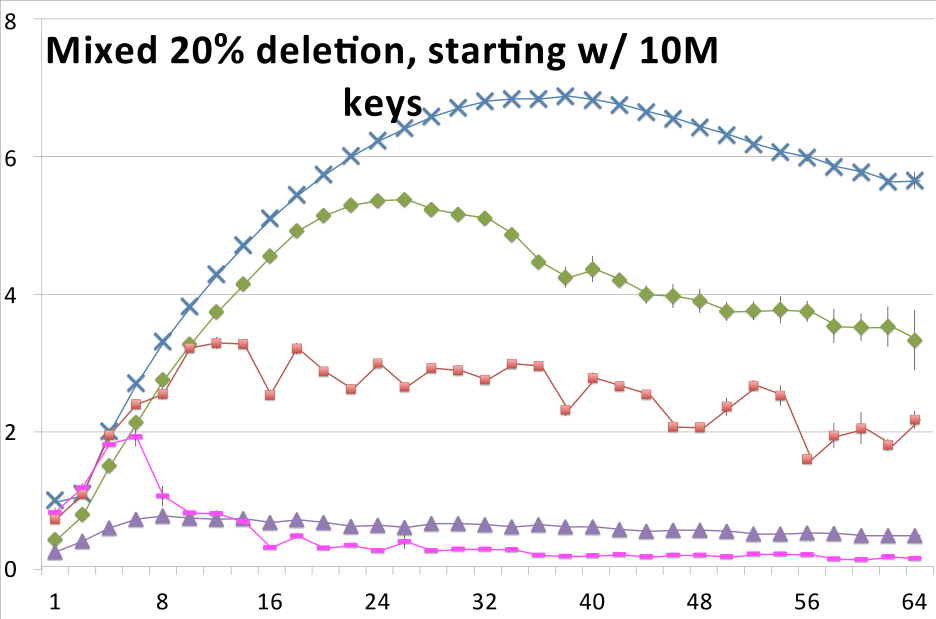
\includegraphics[width=\linewidth]{graphics/cbpq_80add_20.png}
		\caption{Priority queue performance with 80\% \texttt{add()}s, 20\% \texttt{removeMin()}s \cite{braginsky_cbpq:_2016}.}
		\label{fig:cbpq_80}
	\end{minipage}
	\begin{minipage}[b]{.495\textwidth}
		\centering
		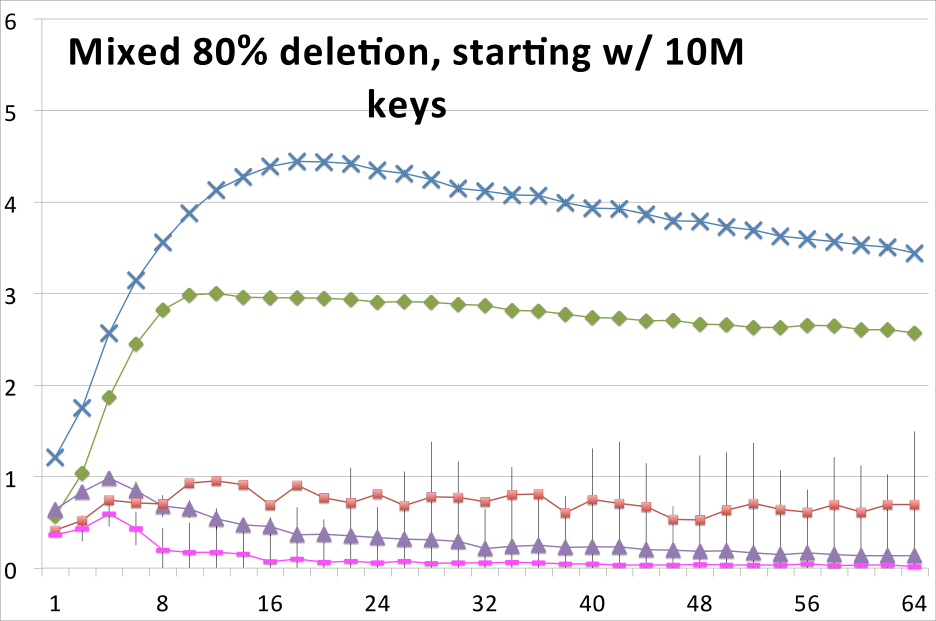
\includegraphics[width=\linewidth]{graphics/cbpq_20add_80.png}
		\caption{Priority queue performance with 20\% \texttt{add()}s, 80\% \texttt{removeMin()}s \cite{braginsky_cbpq:_2016}.}
		\label{fig:cbpq_20}
	\end{minipage}
\end{figure}

\subsection{Evaluation Remarks}
While reading the original papers evaluation a few odd things came up. The Sun SPARC T5240 machine used for cunducting the experiments was introduced in 2008 while the paper was published in 2014. The Intel Xeon they This machine would support up to 128 threads although only up 64 were used in the experiments which means the whole second processer was never used.
\improve{Distribution of priorities inserted?}
\improve{Shortcomings of different algorithms, scenarios where they work good bad and why, what was done to overcome these}

\improve{Criticise why use this machine? seems quite old? why no more threads? why hide compiler details and os? why not all evaluate on the Intel machine? Why these thread counts (increase of 1-2-3-8-8-8-8-8-8-6), use same scaling and especially on x axis a uniform scaling would be better as well}




